\documentclass[a4paper,11pt]{report}

\usepackage{amsmath}
\usepackage{fullpage}
\usepackage{tikz}

\usetikzlibrary{graphs,graphs.standard}

\makeatletter
\pgfmathdeclarefunction{alpha}{1}{%
  \pgfmathint@{#1}%
  \edef\pgfmathresult{\pgffor@alpha{\pgfmathresult}}%
}

\usepackage{bussproofs}
\usepackage{mathpartir}
\usepackage{prooftrees}
\usepackage{color}

\usepackage{tikz}
\usetikzlibrary{automata,positioning}

\author{Sylvain Julmy}
\date{\today}

\setlength{\parindent}{0pt}

\begin{document}

\begin{center}
  \Large{
    Mathematical Methods for Computer Science 1\
    Fall 2017
  }
  \noindent\makebox[\linewidth]{\rule{\linewidth}{0.4pt}}

  Series 9
  \vspace*{1.4cm}

  Sylvain Julmy
  
  \noindent\makebox[\linewidth]{\rule{\linewidth}{0.4pt}}
\end{center}

\section*{\texttt{1}}

\subsection*{\texttt{(a)}}

Let $w \in L$, where  $L = \{\omega \in \{0,1\}* | l_0(\omega) > l_1
(\omega)\}$. We assume $L$ is regular, then there must be some decomposition $w
= xyz$ with $|xy| \leq p$ and $|y| \geq 1$ such that $xy^iz$ in $L$ for every $i
\geq 0$.

We consider the string $w = 0^a1^b$ where $a > b$, $w \in L$ and $|x| \geq n$.
So by the Pumping Lemma, $\exists x,y,z$ such that the Pumping Lemma hold.

Then $w = 0^a1^b = xyz$ with $|xy| \geq n$ and $|y| \geq 1$. So $x = 0^s, y =
0^t, z = 0^u1^v$ with $s+t \leq n$, $t \geq 1$, $u \geq 0$ and $s + t + u > v$.
Then, for $i = 0$, we have :

\[
  xy^iz = xz = 0^t0^v1^u = 0^{t+v}1^u \not\in L
\]

So if $xyz \in L$, then $xz \not\in L$, since $xz$ has fewer $0$ than $xyz$ but
the same number of $1$.So the Pumping Lemma don't hold.

\subsection*{\texttt{(b)}}

The following DFA accept the langage $\{\omega \in \{0,1\}* | l_0(\omega)\text{
  is even}, l_1(\omega)\text{ is odd} \}$.


\begin{center}
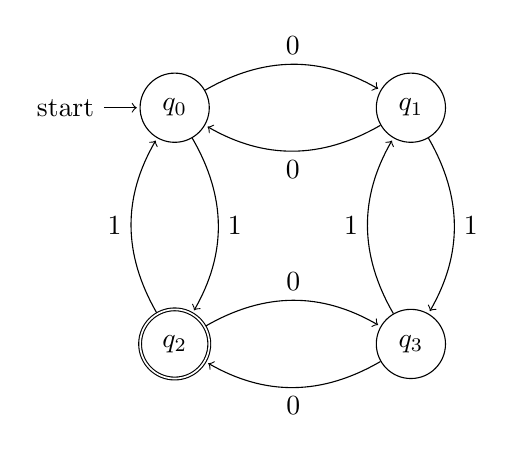
\begin{tikzpicture}[shorten >=1pt,node distance=3cm,on grid,auto]
  \node[state,initial] (q0) {$q_0$};
  \node[state] (q1) [right = of q0] {$q_1$};
  \node[state,accepting] (q2) [below = of q0] {$q_2$};
  \node[state] (q3) [below = of q1] {$q_3$};
  \path[->]
  (q0)
  edge [bend left] node [] {$0$} (q1)
  edge [bend left] node [] {$1$} (q2)
  (q1)
  edge [bend left] node [] {$0$} (q0)
  edge [bend left] node [] {$1$} (q3)
  (q2)
  edge [bend left] node [] {$0$} (q3)
  edge [bend left] node [] {$1$} (q0)
  (q3)
  edge [bend left] node [] {$0$} (q2)
  edge [bend left] node [] {$1$} (q1)
  ;
\end{tikzpicture}
\end{center}

\subsection*{\texttt{(c)}}

Let $w \in L$, where  $L = \{\omega \in \{0,1\}* | l_0(\omega) \neq l_1
(\omega)\}$. We assume $L$ is regular, then there must be some decomposition $w
= xyz$ with $|xy| \leq p$ and $|y| \geq 1$ such that $xy^iz$ in $L$ for every $i
\geq 0$.

We consider the string $w = 0^a1^b$ where $a < b$, $w \in L$ and $|x| \geq n$.
So by the Pumping Lemma, $\exists x,y,z$ such that the Pumping Lemma hold.


Then $w = 0^a1^b = xyz$ with $|xy| \geq n$ and $|y| \geq 1$. So $x = 0^s, y =
0^t, z = 0^u1^v$ with $s+t \leq n$, $t \geq 1$, $u \geq 0$ and $s + t + u < v$.

Now, if we reapet $i$ a certain number of time, we obtain a string where $s + t
+ u = v$ which is not in $L$. Therefore $L$ is not regular.


\section*{\texttt{2}}

\subsection*{\texttt{(a)}}

The minimum number of states of the DFA that accepts the langage of all binary
words whose tenth letter is 0, is $11$, since we have to count the move inside
de word in order to accept a word of $L$ or not. Now we consider a automaton $M$
with $10$ states, then with each transition from $q_i$ to $q_{i+1}$, we can
count a letter in the word, and only one.

The proof is by induction on the number of states $n$:
\paragraph{Base case 1 : $n = 1$} Clearly, with only on state we can't count
anything for a word, because transition only occurs between the initial state
and itself.
\paragraph{Base case 2 : $n = 2$} With $2$ states, we can count $1$ element in
the word, since we don't have any memory, when we go back to the initial state
from the second one, we don't know how many times the transition has been taken,
we can only know that it has been a transition from the initial state to the
second one.

\paragraph{Inductive step :} with $m$ states, we can count $m-1$ transition,
each time a transition is taken from $q_i$ to $q_{i+1}$. When going back from a
state $q_j$ to $q_i$ where $j > i$, we can't make any assumption about the
number of times this transition is taken. But if there are no back transition
from a state $q_j$ to a state $q_i$ where $j > i$, we can, in a way, do some
counting on constant.

\subsection*{\texttt{(b)}}

No idea...

\section*{\texttt{3}}

\subsection*{\texttt{(a)}}

We have $\omega = z_1z_2z_3 = z_1uvwz_3$ and the Pumping
Lemma hold, since $u$ and $w$ can be seen as substring of $z_1$, respectively
$z_3$ (we consider the Pumping Lemma for a string $abc$ where $a = z_1u$, $b =
v$ and $c = wz_3$). There are no condition on the length of $u$ and $w$,
therefore if both length is $0$, this is just the Pumping Lemma.

\subsection*{\texttt{(b)}}

In order to prove that $L = \{a^ib^jc^j | i,j \geq 0\}$ is non regular, we will show
that $L' = \{b^jc^j | j \geq 0\}$ is non regular. Then, by definition, $L$ is
non regular too.

$L' = \{b^jc^j | j \geq 0\}$ is non regular :

We assume that $L$ is regular, then the Pumping Lemma must hold. Let $w =
b^nc^n$, therefore $x \in L'$ and $|x| \geq n$, so by the Pumping Lemma,
$\exists u,v,w$ such that

\begin{gather}
  x = uvw \\
  |uv| \leq n \\
  |v| \geq 1 \\
  \forall i \geq 0 : uv^iw \in L'
\end{gather}

We show that $\forall u,v,w$, (1) to (4) don't hold. If (1) to (3) hold, then $x
= b^nc^n = uvw$ with $|uv| \leq n$ and $|v| \geq 1$. Therefore $u = b^s, v =
b^t, w = b^pc^n$ with $s + t \leq n$, $t \geq 1$, $p \geq 0$, $s+t+p = n$. But
here (4) don't hold for $i=0$ :

\[
  uv^0w = uw = b^sb^pc^n = b^{s+p}c^n \not\in L', \text{ since } s+p \neq n
\]

Finally, $L$ in non regular because $L'$ is non regular.

\section*{\texttt{4}}

\subsection*{\texttt{(a)}}

\begin{gather*}
  \Sigma = \{a,b,c\} \\
  \Delta = \{0,1\} \\
  h : \Sigma^* \mapsto \Delta^* \\
  h(a) = 0, h(b) = 01, h(c) = 10 \\
  L = (a+b)^* + (a+c)^* \\
  h(L) = L' = (0+01)^* + (0+10)^* \\
\end{gather*}

$L'$ do not contains repeating $1$'s and don't start and end with a $1$ at the
same time.

In order to construct a string in $L'$, we have to choose one of the two branch
:

\paragraph{$L'' = (0+01)^*$ :} here it's clear that a string $w \in L''$ can't
start with a $1$, since we have to choose either $0$, $01$ or $\epsilon$ to
start the string with. So the second condition hold. Then, we consider a string
$w$ that's end with a $1$, in order to have repeating $1$, we have to pick a
string $w' \in L''$ which start with a $1$, which is not possible because we saw
that $w \in L''$ necessarily start with a $1$ or is empty.

\paragraph{$L''' = (0+10)^*$ :} here, a string $w \in L'''$ can either start
with a $1$ or a $0$ (or be the empty string...), but it is impossible that such
a string end with a $0$, since both branch of the $+$ are ending with a $0$. So
the second condition hold. Then, in order to have repeating $1$, we have to
append $10$ to a string $w' \in L'''$ that end with a $1$, which is not possible
because we saw that $w \in L'''$ necessarily end with a $0$ or is empty.

\paragraph{} Therefore, $L' = L'' + L'''$ fullfil the conditions.

\subsection*{\texttt{(b)}}

\begin{gather*}
  \Delta = \{0,1\} \\
  h : \Sigma^* \mapsto \Delta^* \\
  L = 0(01)^* \\
  h^{-1}(L) \subset \Sigma^*
\end{gather*}

We can either pick
\[
  h(a) = 0, h(b) = 10
\]

or
\[
  h(a) = 0, h(b) = 01
\]

since $0(10)^*$ and $(01)^*0$ describe the same regular expression.


\begin{gather*}
  \Delta = \{0,1\} \\
  h : \Sigma^* \mapsto \Delta^* \\
  L = 0(01)^* \\
  h^{-1}(L) \subset \Sigma^* \\
  h(a) = 0, h(b) = 10 \\
  h'(a) = 0, h'(b) = 01 \\
  h(L) = ab^* \\
  h'(L) = b^*a \\
  h'(L) = h(L)\\
  h^{-1}(L) = \text{all binary word that start and end with a $0$ and with
    alternating $0$ and $1$}
\end{gather*}

\section*{\texttt{5}}

$L$ is closed under reverse.

Assume $L$ is defined by a regular expression $E$, then we show that there is
another regular expression $rev(E)$ such that $L(rev(E)) = rev(L(E))$, where
$rev(E)$ is the reversal of the langage of $E$.

The proof is by induction on $E$ :

\paragraph{Base case :} if $E = \epsilon$, then it's clear that $rev(E) =
rev(\epsilon) = \epsilon = E$.
\paragraph{Inductive step :} there are three cases depending on $E$ :

\begin{enumerate}
\item $E = F + G$, then $rev(E) = rev(F) + rev(G)$ : the reverse of the union of
  two languages is obtain by taking the union of the reversal of these languages.
\item $E = FG$, the $rev(E) = rev(G)rev(F)$ : the reverse of the concatenation
  of two languages is the concatenation of their reversal.
\item $E = F^*$, then $rev(E) = rev(F)^*$ : any string $w \in rev(F)^*$ is of
  the form $w_1w_2 \dots w_n$ where $w_i$ is the reversal of a string in $F$.
  Therefore $rev(w) = rev(w_1)rev(w_2)\dots rev(w_n)$ and $rev(w_i) \in rev(E)$,
  so $rev(w) \in rev(F)^*$
\end{enumerate}

We can also construct a DFA $M'$ from the DFA $M$ that recognize $L$ in order to
recognize $L' = rev(L)$, by

\begin{itemize}
\item Reversing all arcs.
\item Make the initial state of $M$ the new unique accepting state.
\item Create a new initial state $q_0'$ with $\delta(q_0',\epsilon) = F$.
\end{itemize}

\end{document}
